\section{Modeling and Managing ATSs - The CATSM Problem} 

% ==================///==================///==================///
\begin{frame}{How can ATSs be Modeled?}
	Three main elements to model
	\vspace{0.5cm}
	\begin{itemize}
		\item Road Network
		\item Vehicles
		\item Requests
	\end{itemize}
	\vspace{0.5cm}
	$\rightarrow$ Forming a vehicle-centric model of the ATS
\end{frame}

% ==================///==================///==================///
\begin{frame}{Modeling the Road Network}
	Using a irect graph $\mathcal{G} = \langle \mathcal{V}, \mathcal{E} \rangle$, where $\mathcal{V}$ is the set of vertices (Locations) and $\mathcal{E} \subseteq \mathcal{V} \times \mathcal{V}$ the edges (Roads)
	\vspace{0.5cm}
	\begin{itemize}
		\item Each edge associated with multiple metrics (e.g. distance $d: \mathcal{E} \rightarrow \mathbb{R}_{\geq 0}$)
		\item Nodes can be of two types, charging ($\mathcal{V}_c$) and normal ($\mathcal{V}_n$) nodes 
		\item Charging nodes with different charging profiles
	\end{itemize}
	\vspace{0.5cm}
	Forming a vehicle-centric model of the ATS
\end{frame}


% ==================///==================///==================///

\begin{frame}{Charging Profiles}
	AV batteries modeled using the CC-CV (Constant current - Constant Voltage ) scheme. \\
	Modeled as tuple  $\mathcal{T}_a =\langle Q_a, I^b_a, R^-_a, R^+_a,\theta_a\rangle$. 
	\vspace{0.1cm}
	\input{img/half_battery_profiles}
\end{frame}

% ==================///==================///==================///

\begin{frame}{Modeling AVs}
	Each vehicle $a \in\mathcal{A}$ as a tuple $\langle \underline{s_a},\bar{t_a}, B_a(t),\mathcal{R}_a, \mathcal{T}_a, P_a, G_a, C_a, F_a  \rangle$.
	\begin{itemize}
		\item Starting and terminating depot $\underline{s_a}$ and $\bar{t_a}$ 
		\item  State of Charge $B_a \in \mathbb{R}_{>0}$ at time $t$
		\item  Goods and people capacity $G_a \in \mathbb{R}_{\ge0}$ and $P_a \in \mathbb{R}_{\ge0}$ 
		\item  Operational cost $C_a \in \mathbb{R}_{>0}$ 
		\item  Pollution factor $F_a \in \mathbb{R}_{>0}$
		\item A battery $\mathcal{T}_a$
		%\item Charging and discharching rate $R^-_a, R^+_a$ 
		\item Set of assigned requests $\mathcal{R}_a$ 
	\end{itemize}
\end{frame}

% ==================///==================///==================///

\begin{frame}{Modeling Requests}
	Requests are modeled as tuples $\langle \underline{s'},\bar{t'}, G', P',\lambda, a', b'\rangle$
	\begin{itemize}
		\item  Pick-up and drop-off point $\underline{s'} \in \mathcal{V}_n,\bar{t'} \in \mathcal{V}_n$ 
		\item  Transportation demands for goods and people $G'\in \mathbb{R}_{\ge0}$ $P'\in \mathbb{R}_{\ge0}$ 
		\item  Request arrival rate $\lambda \in \mathbb{R}_{>0}$ 
		\item  Time window $[a',b']$ 
	\end{itemize}
\end{frame}

% ==================///==================///==================///
\begin{frame}{Leveraging the Request Model}
	Requests are key to solve the rebalancing problem
	\begin{columns}
		\begin{column}{0.4\textwidth}
				
			\begin{itemize}
				\item  Exploiting $\lambda$
				\item   Division in regions around depots, i.e. $\mathcal{G}_v = \langle \mathcal{V}'_v, \mathcal{E}'_v\rangle$
				\item 	Rebalancing becomes fundamentally an assignment problem 
			\end{itemize}
		\end{column}
		\begin{column}{0.5\textwidth}
			\begin{figure}
				\centering
					\resizebox{1\textwidth}{!}{
				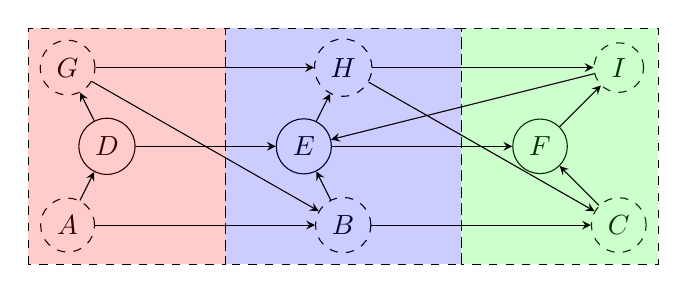
\begin{tikzpicture}[>=stealth]
					
					% Draw rectangle
					%\draw (-1,0) rectangle (8,4);
					
					% Nodes
					\foreach \x/\y/\n in {0/1/A, 3.5/1/B, 7/1/C,  0/3/G, 3.5/3/H, 7/3/I} {
						\node[dashed, circle, draw, fill=white] (\n) at (\x, \y) {$\n$};
					}
					
					\foreach \x/\y/\n in { 0.5/2/D, 3/2/E, 6/2/F} {
						\node[circle, draw, fill=white] (\n) at (\x, \y) {$\n$};
					}
					
					
					% Groups
					\draw[dashed, fill=red, fill opacity=0.2] (-0.5,0.5) rectangle (2,3.5);
					\draw[dashed, fill=blue, fill opacity=0.2] (2,0.5) rectangle (5,3.5);
					\draw[dashed, fill=green, fill opacity=0.2] (5,0.5) rectangle (7.5,3.5);
					
					% Arrows
					\foreach \from/\to in {A/B, B/C, D/E, E/F, G/H, H/I, A/D, B/E, C/F, D/G, E/H, F/I, G/B, H/C, I/E} {
						\draw[->] (\from) -- (\to);
					}
				\end{tikzpicture}
			}
			\end{figure}
			\begin{center}
				$\mathcal{R}_v'= \{ r \in \mathcal{R} : \underline{s_r}' \in \mathcal{V'}_v \} \label{eq:req_per_reg}$
			\end{center}
			
		\end{column}
	\end{columns}

\end{frame}

% ==================///==================///==================///

\begin{frame}{The Complete ATS Management Problem}
	In a nutshell, maximize number of served requests and minimize vehicle's travel time, while
	\begin{itemize}
		\item Respecting deadlines
		\item Observing vehicle's characteristics (e.g. charge and capacity)
		\item  Eliminating congestions $\rightarrow$ artificial limit $c$ on vehicles per road.
	\end{itemize}
\end{frame}
% ==================///==================///==================///

\begin{frame}{Simulating the CATSM in Real-World}
	 \begin{columns}
	 		\begin{column}{0.37\textwidth}
	 			Using real-world data from NYC\\
	 			\begin{itemize}
	 				\item Simplified, yet large road network ($|\mathcal{V}|=$~500, $|\mathcal{E}|=$1700 )
	 				\item Fictitious depots' locations
	 				\item Deterministic requests rates
	 	 		\end{itemize}
	 		\end{column}
	 			\begin{column}{0.44\textwidth}
	 			\begin{figure}[tbh]
	 				\centering
	 				\begin{tikzpicture}[node distance=0cm]
	 					\node (left) at (0,-1) {\includegraphics[width=0.45\textwidth]{img/new_york_vanilla_info.png}};
	 					\node[right=0.1cm of left, scale=2] {$\Rightarrow$};
	 					\node (right) at (4,-1) {\includegraphics[width=0.45\textwidth]{img/new_york_simplified_roads.png}};
	 				\end{tikzpicture}
	 			\end{figure}
	 			\vspace{0.5cm}
	 		\end{column}
	 \end{columns}
\end{frame}

% ==================///==================///==================///

\begin{frame}{System's Performance in a Nutshell}

			\begin{table}[h]
				\centering
				\begin{tabular}{ |p{3.7cm}|c|c|c|c|}
					\cline{2-5}
					\multicolumn{1}{c}{}&\multicolumn{2}{|c|}{w/o Rouing} &\multicolumn{2}{|c|}{w/ Routing}\\
					\cline{2-5}
					\multicolumn{1}{c|}{}& Sim. 1 & Sim. 2 & Sim. 1 & Sim. 2\\
					\hline
					Total Distance (m) &731993& 749006& 806280&874937\\
					Average Distance (m) &30500 & 312089 &33595&36456\\
					Total Time (s) &14640& 14980 &16126&17499\\
					Average Time (s) & 610& 624 &672&729\\
					Unique Road Used &1171&1137 &1193&1206\\
					Request Served (\%)&64 & 63 &81&78\\
				\end{tabular}
			\end{table}
\end{frame}
% ==================///==================///==================///
\begin{frame}{Evaluation}
	\hspace{0.5cm} Promising results, but interrogatives are left open. 
	\vspace{0.5cm}
	\begin{columns}
		\begin{column}{0.35\textwidth}
			\begin{itemize}
				\item[+] Solves all the ATSs challenges
				\item[+] Finds numerically optimal solutions
				\item[+] Is flexible and modular
			\end{itemize}
		\end{column}
		%%
		\vline
		\hspace{0.8cm}
		\begin{column}{0.4\textwidth}
			\begin{itemize}
				\item[-] Congestions' model is highly simplified
				\item[-] Suffers large networks
				\item[-] Is not suitable for real-time 
				\item[-] Doesnt have possible insights on the future
			\end{itemize}
		\end{column}
	\end{columns}
\end{frame}